\section{Suddivisione del lavoro e prospetto orario}
Ogni componente del gruppo dovrà ricoprire ogni ruolo almeno una volta nel corso del progetto.
Durante lo stesso periodo un componente può ricoprire più ruoli, a condizione che le mansioni previste non vadano in conflitto tra loro, ad esempio non si può verificare il proprio lavoro.
Segue il prospetto orario suddiviso per periodi e totale. \\

Nell'intestazione utilizzata per le tabelle di questo capitolo sono state impiegate \textbf{abbreviazioni} per i nomi dei ruoli.
Di seguito viene riportato il loro significato, \textbf{nell'ordine in cui sono utilizzate} nell'intestazione:
\begin{itemize}
\item Amm.: \textit{Amministratore};
\item Ana.: \textit{Analista};
\item Pgt.: \textit{Progettista};
\item Pgr.: \textit{Programmatore};
\item Res.: \textit{Responsabile};
\item Ver.: \textit{Verificatore}.
\end{itemize}

%-----------------------------------------------------------------------------------------------------
%-------------------------------------- ANALISI ------------------------------------------------------
%-----------------------------------------------------------------------------------------------------
\pagebreak
\subsection{Analisi}
Nel periodo di Analisi dei requisiti ciascun componente dovrà rivestire i seguenti ruoli:

\begin{table}[H]
\begin{tabular}{lccccccc}
\toprule
    \textbf{Nome}  & \multicolumn{6}{c}{\textbf{Ore per ruolo}} & \textbf{Ore totali} \\
     & Amm. & Ana. & Pgt. & Pgr. & Res. & Ver. & \\
    \midrule
    
	Andrea Mantovani & 12 & 0 & 0 & 0 & 11 & 0 & 23 \\
	Davide Polonio & 16 & 0 & 9 & 0 & 0 & 0 & 25 \\
	Davide Rigoni & 0 & 12 & 0 & 0 & 0 & 8 & 20 \\
	Emanuele Carraro & 0 & 15 & 0 & 0 & 0 & 6 & 21 \\
	Giovanni Mazzocchin & 0 & 11 & 0 & 0 & 0 & 11 & 22 \\
	Luca Bianco & 0 & 12 & 0 & 0 & 0 & 8 & 20 \\
	Matteo di Pirro & 0 & 0 & 4 & 0 & 18 & 0 & 22 \\
    %totale ore: 153 
    
    \bottomrule
\end{tabular}
\caption{Ore per componente, fase di Analisi}
\end{table}


I valori in tabella sono riassunti nel seguente grafico: \\ 

    \begin{figure}[H]
      \begin{center}
        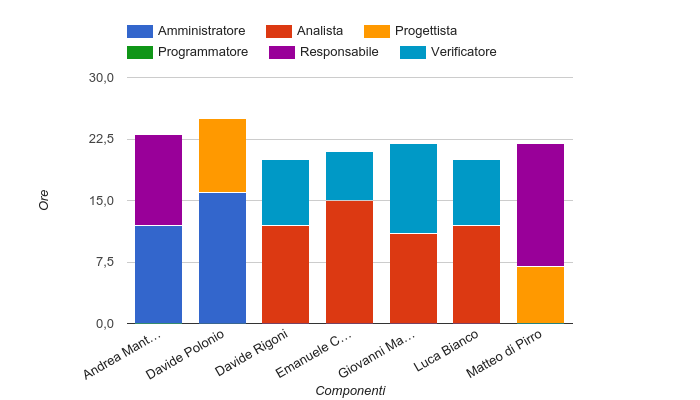
\includegraphics[width=12cm]{res/img/orePerComponenteAnalisi.png}
      \caption{Ore per componente, fase di Analisi}
      \end{center} 
    \end{figure}    
    
Si fa notare che le ore sopra indicate non sono incluse nelle 105 ore rappresentanti il tetto massimo di ore somministrabile da ciascun componente.


%-----------------------------------------------------------------------------------------------------
%-------------------------------------- PROGETTAZIONE ARCHITETTURALE ---------------------------------
%-----------------------------------------------------------------------------------------------------
\pagebreak
\subsection{Progettazione Architetturale}
Nella fase di Progettazione architetturale ciascun componente dovrà rivestire i seguenti ruoli:

\begin{table}[H]
\begin{tabular}{lccccccc}
\toprule
    \textbf{Nome}  & \multicolumn{6}{c}{\textbf{Ore per ruolo}} & \textbf{Ore totali} \\
     & Amm. & Ana. & Pgt. & Pgr. & Res. & Ver. & \\
    \midrule
    
	   Andrea Mantovani & 0 & 5 & 19 & 0 & 0 & 7 & 31 \\
         Davide Polonio & 0 & 0 & 21 & 0 & 0 & 3 & 24 \\
       	  Davide Rigoni & 8 & 0 & 19 & 0 & 0 & 3 & 30 \\
	   Emanuele Carraro & 7 & 0 & 11 & 0 & 0 & 4 & 22 \\
	Giovanni Mazzocchin & 0 & 0 & 10 & 0 & 6 & 15 & 31 \\
	        Luca Bianco & 0 & 0 & 21 & 0 & 0 & 8 & 29 \\
      	Matteo di Pirro & 0 & 0 & 18 & 0 & 0 & 14 & 32 \\
           %totale ore: 199
    
    \bottomrule
\end{tabular}
\caption{Ore per componente, fase di Progettazione architetturale}
\end{table}

I valori in tabella sono riassunti nel seguente grafico: \\ 

    \begin{figure}[H]
      \begin{center}
        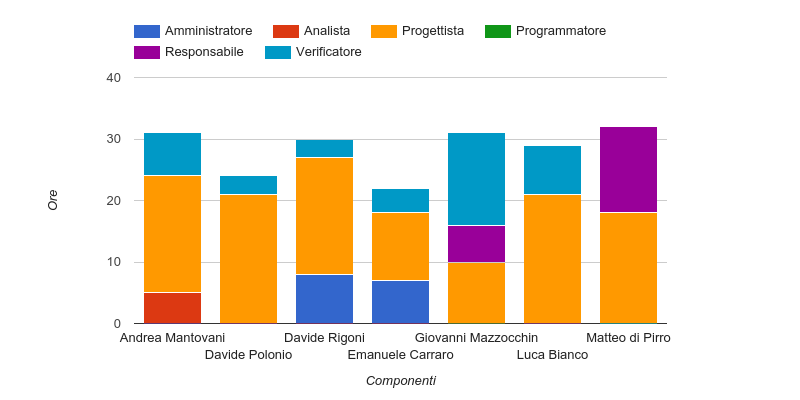
\includegraphics[width=12cm]{res/img/orePerComponenteProgettazioneArchitetturale.png}
      \caption{Ore per componente, fase di Progettazione architetturale}
      \end{center} 
    \end{figure}    
    
    
    
    
%-----------------------------------------------------------------------------------------------------
%-------------------------------------- PROGETTAZIONE DI DETTAGLIO E CODIFICA ------------------------
%-----------------------------------------------------------------------------------------------------
\pagebreak
\subsection{Progettazione di dettaglio e codifica}
Nella fase di Progettazione di dettaglio e codifica ciascun componente dovrà rivestire i seguenti ruoli:

\begin{table}[H]
\begin{tabular}{lccccccc}
\toprule
    \textbf{Nome}  & \multicolumn{6}{c}{\textbf{Ore per ruolo}} & \textbf{Ore totali} \\
     & Amm. & Ana. & Pgt. & Pgr. & Res. & Ver. & \\
    \midrule
    
	Andrea Mantovani & 0 & 12 & 9 & 0 & 0 & 2 & 23 \\
	Davide Polonio & 0 & 9 & 0 & 0 & 4 & 9 & 22 \\
	Davide Rigoni & 9 & 2 & 0 & 0 & 5 & 4 & 20 \\
	Emanuele Carraro & 0 & 10 & 0 & 0 & 0 & 11 & 21 \\
	Giovanni Mazzocchin & 6 & 11 & 0 & 0 & 0 & 0 & 17 \\
	Luca Bianco & 15 & 0 & 0 & 0 & 5 & 0 & 20 \\
	Matteo di Pirro & 0 & 14 & 0 & 0 & 0 & 5 & 19 \\
    
    \bottomrule
\end{tabular}
\caption{Ore per componente, fase di Progettazione di dettaglio e codifica}
\end{table}

I valori in tabella sono riassunti nel seguente grafico: \\ 

    \begin{figure}[H]
      \begin{center}
        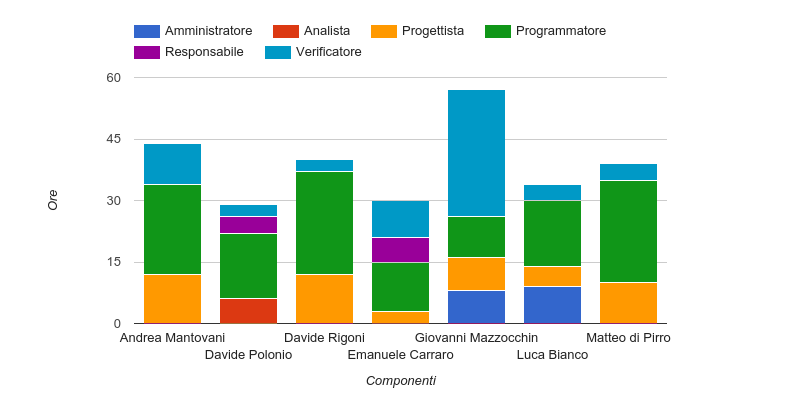
\includegraphics[width=12cm]{res/img/orePerComponenteProgettazioneDettaglioCodifica.png}
      \caption{Ore per componente, fase di Progettazione di dettaglio e codifica}
      \end{center} 
    \end{figure}    
    
    
    
%-----------------------------------------------------------------------------------------------------
%-------------------------------------- VALIDAZIONE --------------------------------------------------
%-----------------------------------------------------------------------------------------------------
\pagebreak
\subsection{Validazione}
Nella fase di Validazione ciascun componente dovrà rivestire i seguenti ruoli:

\begin{table}[H]
\begin{tabular}{lccccccc}
\toprule
    \textbf{Nome}  & \multicolumn{6}{c}{\textbf{Ore per ruolo}} & \textbf{Ore totali} \\
     & Amm. & Ana. & Pgt. & Pgr. & Res. & Ver. & \\
    \midrule
    
	Andrea Mantovani & 8 & 0 & 15 & 0 & 0 & 0 & 23 \\
	Davide Polonio & 15 & 0 & 6 & 0 & 0 & 0 & 21 \\
	Davide Rigoni & 0 & 12 & 0 & 0 & 0 & 7 & 19 \\
	Emanuele Carraro & 0 & 16 & 0 & 0 & 0 & 7 & 23 \\
	Giovanni Mazzocchin & 0 & 11 & 0 & 0 & 0 & 10 & 21 \\
	Luca Bianco & 0 & 10 & 0 & 0 & 0 & 12 & 22 \\
	Matteo di Pirro & 0 & 0 & 5 & 0 & 15 & 0 & 20 \\
    
    \bottomrule
\end{tabular}
\caption{Ore per componente, fase di Verifica}
\end{table}

I valori in tabella sono riassunti nel seguente grafico: \\ 

    \begin{figure}[H]
      \begin{center}
        \includegraphics[width=12cm]{res/img/orePerComponenteVerifica.png}
      \caption{Ore per componente, fase di Verifica}
      \end{center} 
    \end{figure}    
    
    
    
%-----------------------------------------------------------------------------------------------------
%-------------------------------------- TOTALE -------------------------------------------------------
%-----------------------------------------------------------------------------------------------------
\pagebreak
\subsection{Totale}
Il totale delle ore, comprensive delle ore di Analisi dei requisiti che saranno fornite da ciascun membro
del gruppo nel corso dell’intero progetto sono le seguenti:

\begin{table}[H]
\begin{tabular}{lccccccc}
\toprule
    \textbf{Nome}  & \multicolumn{6}{c}{\textbf{Ore per ruolo}} & \textbf{Ore totali} \\
     & Amm. & Ana. & Pgt. & Pgr. & Res. & Ver. & \\
    \midrule
    
	Andrea Mantovani & 0 & 12 & 9 & 0 & 0 & 2 & 23 \\
	Davide Polonio & 0 & 9 & 0 & 0 & 4 & 9 & 22 \\
	Davide Rigoni & 9 & 2 & 0 & 0 & 5 & 4 & 20 \\
	Emanuele Carraro & 0 & 10 & 0 & 0 & 0 & 11 & 21 \\
	Giovanni Mazzocchin & 6 & 11 & 0 & 0 & 0 & 0 & 17 \\
	Luca Bianco & 15 & 0 & 0 & 0 & 5 & 0 & 20 \\
	Matteo di Pirro & 0 & 14 & 0 & 0 & 0 & 5 & 19 \\
    
    \bottomrule
\end{tabular}
\caption{Ore per componente totali, inclusa la fase di Analisi}
\end{table}

I valori in tabella sono riassunti nel seguente grafico: \\ 

    \begin{figure}[H]
      \begin{center}
        \includegraphics[width=12cm]{res/img/orePerComponenteTotaliAnalisi.png}
      \caption{Ore per componente totali, inclusa la fase di Analisi}
      \end{center} 
    \end{figure}    
    
Nella seguente tabella sono invece riportate le ore fornite da ciascun componente, escluse quelle rientranti nella fase di Analisi dei requisiti.

    \begin{table}[H]
    \begin{tabular}{lccccccc}
    \toprule
        \textbf{Nome}  & \multicolumn{6}{c}{\textbf{Ore per ruolo}} & \textbf{Ore totali} \\
         & Amm. & Ana. & Pgt. & Pgr. & Res. & Ver. & \\
        \midrule
        
    	Andrea Mantovani & 0 & 12 & 9 & 0 & 0 & 2 & 23 \\
    	Davide Polonio & 0 & 9 & 0 & 0 & 4 & 9 & 22 \\
    	Davide Rigoni & 9 & 2 & 0 & 0 & 5 & 4 & 20 \\
    	Emanuele Carraro & 0 & 10 & 0 & 0 & 0 & 11 & 21 \\
    	Giovanni Mazzocchin & 6 & 11 & 0 & 0 & 0 & 0 & 17 \\
    	Luca Bianco & 15 & 0 & 0 & 0 & 5 & 0 & 20 \\
    	Matteo di Pirro & 0 & 14 & 0 & 0 & 0 & 5 & 19 \\
        
        \bottomrule
    \end{tabular}
    \caption{Ore per componente, rendicontate}
    \end{table}
    
    I valori in tabella sono riassunti nel seguente grafico: \\ 
    
        \begin{figure}[H]
          \begin{center}
            \includegraphics[width=12cm]{res/img/orePerComponenteTotaliRendicontate.png}
          \caption{Ore per componente, rendicontate}
          \end{center} 
        \end{figure}   
    
